IncBricks \cite{incbricks} is a hardware-software co-designed system for in-network caching: it makes use of network accelerators attached to programmable switches whenever complicated operations should be performed on payloads.
Supporting multiple gigabytes of memory, network accelerators overcome the limited storage problem typical of programmable switches, which usually have a memory of tens of megabytes.

\subsubsection{Details}
\paragraph{Hardware}
IncBricks \cite{incbricks} is composed by two components:
\begin{mylist}
    \item IncBox, an hardware unit consisting of a network accelerator and a programmable switch, and
    \item IncCache, a software system for coherent key-value storage
\end{mylist}.
Packets arriving to an IncBox device are first managed by the switch, which forwards the packet to the network accelerator only if it is labeled as an in-network cache one.

\begin{figure}[!htb]
    \centering
        % trim = left, bottom, right, top
        \includegraphics[page=3, clip, trim=3.6cm 0.7cm 2.5cm 4.15cm, width=1.00\textwidth]{figures/analysis/inp/solutions.pdf}
    \caption{IncBricks' \texorpdfstring{\cite{incbricks}}{} logical communication pattern}
\end{figure}

If there is a match, the programmable switch will check whether the packet has been already cached by the network accelerator or not, and will forward the packet to the right network accelerator attached to it in the former case.

\begin{figure}[!htb]
    \centering
        % trim = left, bottom, right, top
        \includegraphics[page=4, clip, trim=4.1cm 0.1cm 4.3cm 0.1cm, width=1.00\textwidth]{figures/analysis/inp/solutions.pdf}
    \caption{Messages exchanged during an IncBricks \texorpdfstring{\cite{incbricks}}{} instance execution}
\end{figure}

\paragraph{Logic}
The system has been designed having a multi-rooted tree topology in mind.
For each key the centralized \gls{sdn} controller comes up with a set of \textit{designated} IncBox units allowed to cache that key.
Any other IncBox unit placed between these designated units won't cache data with that specific key.
Then, for a given key and a given destination node, the \gls{sdn} controller establishes a unique path of designated IncBox units.
Every IncBox unit in the system will get to know
\begin{mylist}
    \item the set of immediate designated successors (according to the tree topology) for every key it is responsible of and
    \item the unique successor used for a given destination and a given key
\end{mylist}.
This data is stored in the so-called \textit{global registration table}.
Storing the former information can be useful in case of failures since it is possible to build alternative paths immediately, making the whole system more reliable.
As soon as a failure is detected, the \gls{sdn} controller updates all the involved tables.

\subsubsection{Implementation}
The storage has been implemented using a bucket spilling hash table plus a hash index table
\textbf{\textit{TO BE CONTINUED}} ...

\subsubsection{Minimum system requirements}
Communicating nodes (\glspl{vm}) represent the leaves of the tree.
Each path must include exactly one root switch.

\begin{figure}[!htb]
    \centering
        % trim = left, bottom, right, top
        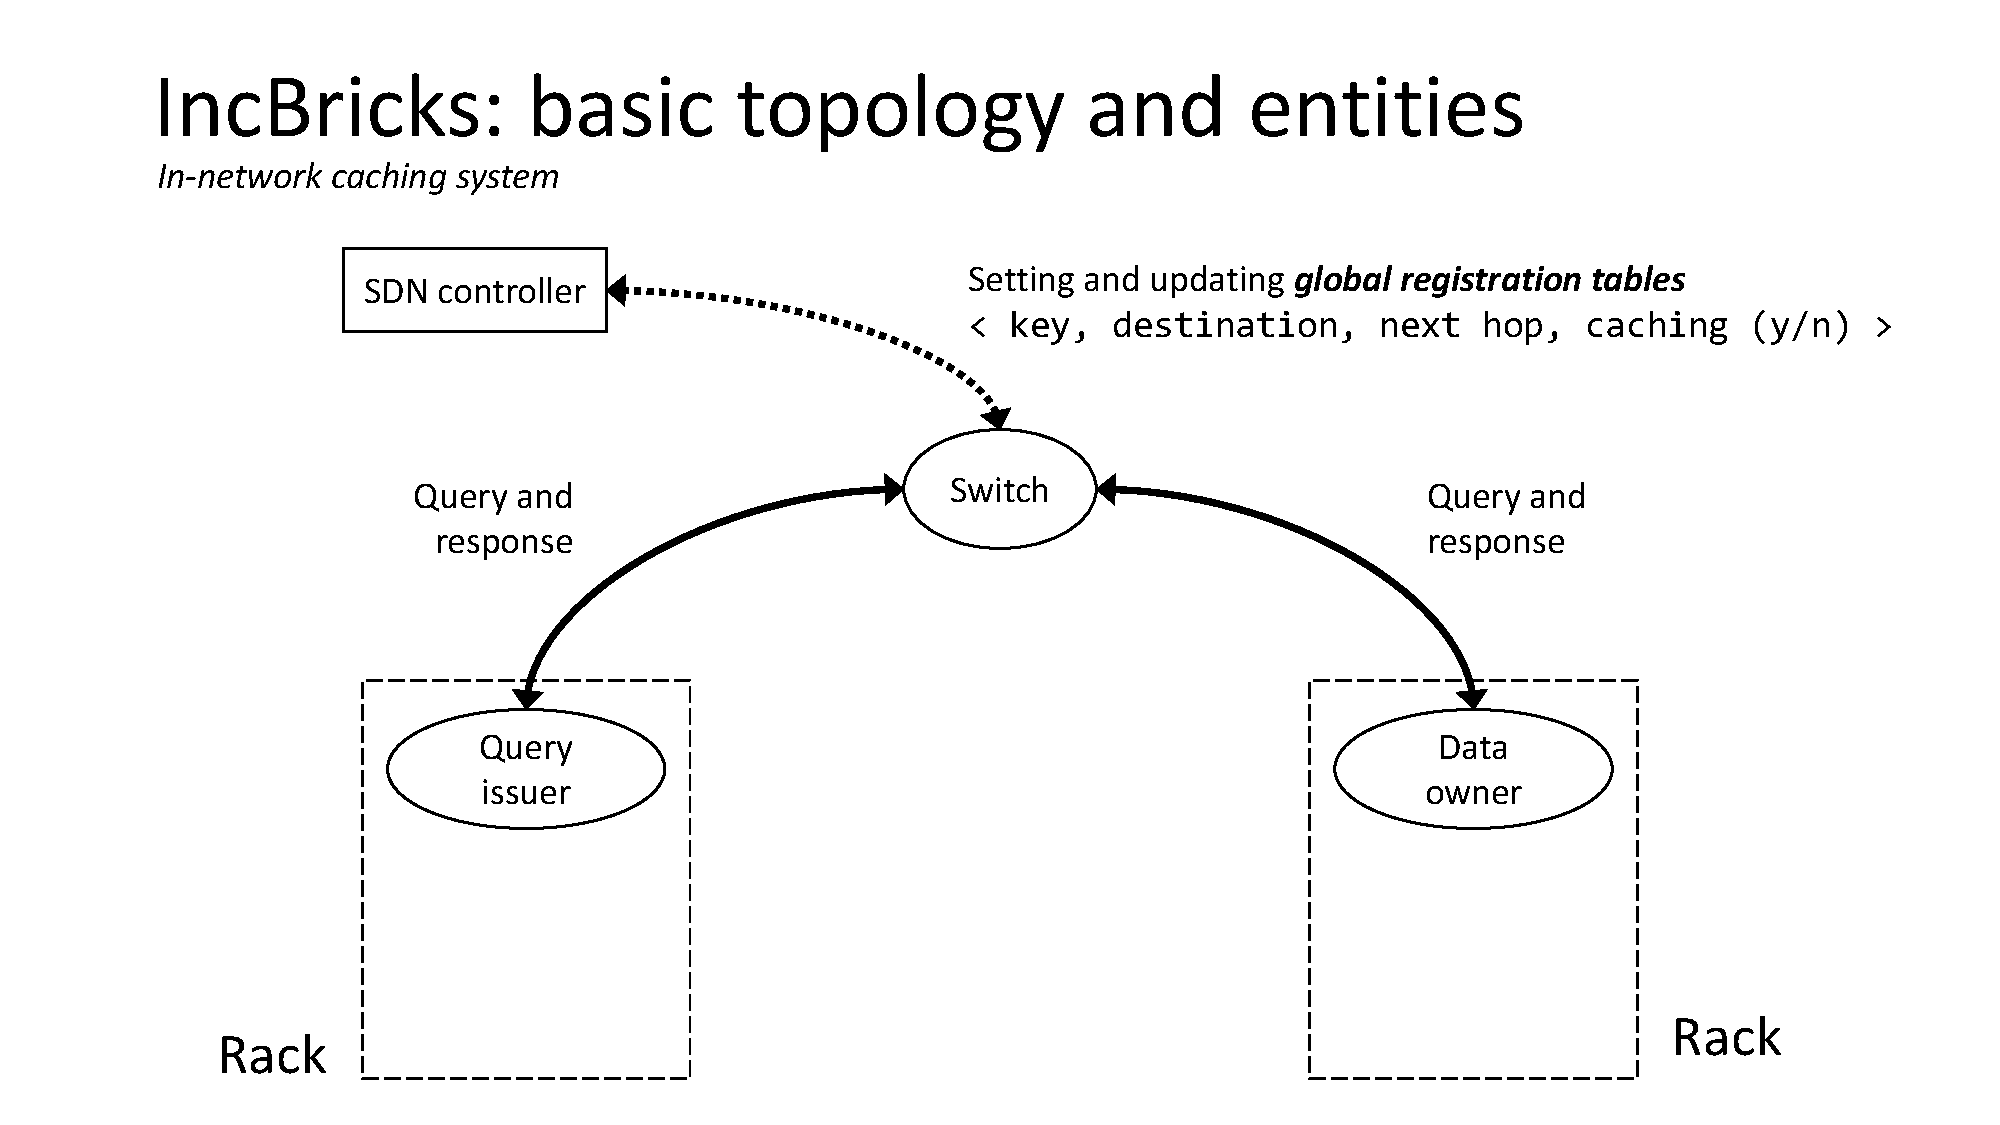
\includegraphics[page=1, clip, trim=3.6cm 0.7cm 2.5cm 4.15cm, width=1.00\textwidth]{figures/analysis/inp/solutions.pdf}
    \caption{IncBricks' \texorpdfstring{\cite{incbricks}}{} basic topology and entities}
\end{figure}

All things considered, it seems reasonable to state that the actual required topology is a chain starting from a leaf, passing through a root node and ending on another leaf.

\begin{figure}[!htb]
    \centering
        % trim = left, bottom, right, top
        \includegraphics[page=2, clip, trim=3.6cm 0.7cm 2.5cm 4.15cm, width=1.00\textwidth]{figures/analysis/inp/solutions.pdf}
    \caption{IncBricks' \texorpdfstring{\cite{incbricks}}{} extended topology}
\end{figure}

IncBox units must dedicate some local storage to realize the caching system.
The solution requires that the system has a centralized \gls{sdn} controller connected to all switches.
The \gls{sdn} controller must set configure network devices in order for them to forward IncBricks \cite{incbricks} packets accordingly.

\subsubsection{Conclusions}